\chapter{The ML2P-VAE Method for IRT Parameter Estimation}\label{ch:ml2pvae_methods}
The primary contribution of this thesis is the development of a method for IRT parameter estimation which uses a modified VAE. The method, titled ``ML2P-VAE'', is interesting from multiple perspectives. In the application area, it is an unconventional approach that produces estimates with similar accuracy of traditional parameter estimation techniques. Further, ML2P-VAE scales much better than traditional methods as the number of latent abilities becomes large. 

In traditional IRT parameter estimation, large datasets present a \textit{burden} -- they require more parameters to be estimated and a larger number of computations. But ML2P-VAE, through the lens of machine learning, views large datasets as a \textit{blessing} -- bigger data provides more information (more responses $u_{ij}$) to learn from in order to more accurately reconstruct inputs. A better reconstruction of input responses directly correlates with improved parameter estimates.

In the field of machine learning, ML2P-VAE is seen as an unsupervised learning technique which yields explainable results. A variational autoencoder is used in an unorthodox way -- VAE are typically used as generative models where only the decoder is used at test-time. In ML2P-VAE, test-time involves feeding student responses through the encoder to obtain a prediction of latent traits -- a result of an interpretable hidden neural network layer. The trainable parameters in the decoder are able to be understood in a real-world context -- they serve as estimates to item parameters to the ML2P model from Section \ref{sec:mirt}. In fact, the entire VAE decoder can be interpreted as an approximate ML2P model (see Equation \ref{eq:ml2p}).

Another important contribution of this thesis is the development of a novel neural network architecture which fits a VAE to a multivariate Gaussian distribution $\mathcal{N}(\vect \mu, \Sigma)$ where the latent code is correlated. This is a significant difference from previous implementations of VAE, which always assume that the dimensions of the latent code are independent of each other (see Equation \ref{eq:ind_gauss_kl}). The more general architecture presented in this thesis is particularly helpful when additional domain knowledge of the latent code is accessible.

\section{ML2P-VAE Method Description}\label{sec:ml2p_vae}
Given an assessment with $n$ items which tests $K$ latent skills, assume that $N$ students take this exam. Data is given as an $N \times n$ binary matrix $U$, as in Equation \ref{eq:responses}. No information about the student latent ability parameters $\vect \Theta \in \R^K$ or the item parameters $a_{ik}$ and $b_i$ is provided. However, assume that there is access to an expert-annotated binary $Q$-matrix detailing the item-skill associations, described by Equation \ref{eq:q_matrix}. Implicitly, we assume that the student responses were generated by the ML2P model, introduced in Equations \ref{eq:ml2p} and \ref{eq:ml2pq}:
\begin{equation}
  P(u_{ij} = 1 | \vect \Theta_j; \vect{a_i}, b_i) = \frac{1}{1 + \exp\left(-\sum_{k=1}^K q_{ik} a_{ik} \theta_{jk} + b_i \right)}
  \label{eq:ml2p_again}
\end{equation}

This assumption directly links IRT with VAE. Recall from Section \ref{sec:vae_derive} that the VAE decoder parameterizes the posterior distribution $p_\beta(\vect x | \vect z)$, seen in Figure \ref{fig:vae_visual}. Replace the observed data $\vect x$ with the student responses $\vect u_j$ and the latent code $\vect z$ with the latent traits $\vect \Theta_j$, and we see that Equation \ref{eq:ml2p_again} provides an explicit form for the posterior distribution $p_\beta(\vect x | \vect z)$ learned by a VAE decoder. Recall that the subscript $\beta$ references a particular setting of the weights in the VAE decoder, drawing parallel with the item parameters $\vect a_i$ and $b_i$. Though $\vect a_i$ and $b_i$ are unknown, the constraints imposed by entries in the $Q$-matrix $q_{ik}$ provide enough structure for the neural network to learn these values during the training process, so long as $Q$ is sufficiently sparse \cite{jiang2018}.

A number of specifications are required in order to use a VAE as an IRT parameter estimation method. First, set up the neural network so that the input and output layers each have $n$ nodes, each node representing one item. The inputs are the binary response vectors $\vect u_j$ defined in Equation \ref{eq:responses} and the outputs are approximations of the probability of student $j$ answering each item correctly. 

The dimension of the hidden distribution (the output of the encoder) must be equal to $K$, the number of latent skills. The usual VAE loss function described in Equation \ref{eq:vae_loss} is still used to optimize ML2P-VAE. The KL-Divergence term acts as a regularizer between the posterior distribution produced by the encoder $q_\alpha(\vect \Theta_j | \vect u_j)$ and prior distribution of latent abilities $p(\vect \Theta)$. Usually, these distributions are assumed to be independent Gaussian, but we extend this idea to a more general multivariate Gaussian distribution where the latent traits $\vect \Theta$ are correlated in Section \ref{sec:cov}.

The modifications to a typical VAE architecture are focused on the decoder. No hidden layers are used in the decoder. Instead, a non-dense matrix of weights connects the decoder input to the decoder output. The non-zero weights here are determined by the binary $Q$-matrix from Equation \ref{eq:q_matrix}; recall that the input to the decoder has $K$ nodes, the decoder output has $n$ nodes, and $Q \in \{0,1\}^{n \times K}$. So for a trainable weight $w_{ik}$ in the VAE decoder, if $q_{ik}=0$, then fix $w_{ik}=0$ as well, and it will never be updated during the training process. This modification is key to allowing interpretation of the hidden latent distribution of a VAE, and is visualized in Figure \ref{fig:ml2pvae_visual}.

The ML2P-VAE method requires the use of the sigmoid activation function
\begin{equation}
  \sigma(z_i) = \frac{1}{1 + e^{-z_i}} = \frac{1}{1 + \exp\left(- \sum_{k=1}^K w_{ik} \alpha_k + \beta_i \right)}
  \label{eq:sigmoid}
\end{equation}
in the output layer (see Appendix \ref{apdx:activation_fcns}). Here, $z_i = \sum_{k=1}^K w_{ik}\alpha_{k} + \beta_i$ is the input to the $i$-th node in the decoder, where $w_{ik}$ is the weight between the $k$-th and $i$-th nodes in the decoder input and decoder output layer and $\beta_i$ is the additive bias in the output layer. $\alpha_k$ is the activation of the $k$-th node in the decoder input layer, which is the sample drawn from the posterior distribution produced by the encoder. 

Note the similarity between Equation \ref{eq:sigmoid} and the ML2P model in Equation \ref{eq:ml2p_again}. The constraint on the weights along with the sigmoid activation function allows for interpretation of the VAE decoder as an approximate ML2P model.

Specifically, the nonzero decoder weights $w_{ik}$ can be interpreted as estimates to the discrimination parameters $a_{ik}$, the output bias $\beta_i$ can be interpreted as estimates to the difficulty parameters $b_i$, and the activations $\alpha_k$ produced by the encoder (given the response input $\vect u_j$) can be interpreted as estimates to the student ability parameter $\theta_{kj}$. All of this explainability is allowed by the constraint on the decoder weights matrix imposed by the binary $Q$-matrix.

Further modifications can improve the performance of ML2P-VAE. In IRT, discrimination parameters are assumed to be non-negative, because an increase in a skill should never decrease the probability of answering an item correctly. With this assumption in mind, requiring all decoder weights $w_{ik} \geq 0$ avoids a potential identification problem, since $\theta^* \cdot a^* = (-\theta^*)\cdot(-a^*)$.

To summarize, the ML2P-VAE model takes as input the student responses $\vect u_j$ and maps them through a VAE encoder to estimates of the student's latent abilities $\vect \Theta_j$. This estimate is sent through a \textit{modified} VAE decoder, whose trainable parameters serve as estimates to the ML2P model. The final output of the VAE decoder is the estimated probability of student $j$ answering each item $i$ correctly, $P_{ij} = \sigma(\vect a_i^\top \vect \Theta_j + b_i)$ as described in Equation \ref{eq:sigmoid}, which is treated as a reconstruction of the inputs $u_{ij}$.


\subsection{Full Covariance Matrix Implementation}\label{sec:cov}
In this section, we detail a novel architecture for a VAE which fits observed data to a latent space with correlated latent code, $\mathcal{N}(\vect \mu, \Sigma)$. There are many publicly available code examples of VAE implementations which assume the latent space follows a standard normal distribution $\mathcal{N}(0,I)$. But it is not so common to train a VAE which assumes that the latent prior $p(\vect \Theta)$ has correlated dimensions. Since most applications do not attempt to interpret hidden layers of a VAE, there is no available information on the correlations of abstract, unobservable features. Additionally, it can be beneficial to force the latent dimensions to be independent of one another when considering the usual applications of VAE.

In IRT, we may be able to quantify the correlation between latent abilities, presenting need for the ML2P-VAE model to take advantage of this information. This task is nontrivial due to two mechanisms of the VAE:
\begin{itemize}
  \item[(1)] sampling from the learned distribution as in Equation \ref{eq:bernoulli}, and
  \item[(2)] calculating Kullback-Leibler Divergence as in Equation \ref{eq:ind_gauss_kl}.
\end{itemize}
These two characteristics must be addressed when constructing a neural architecture which accounts for correlated $\vect \Theta$.

After training a VAE, sending a data point $\vect u_0$ through the encoder needs to give a set of values that correspond to a probability distribution. For a $K$-dimensional multivariate Gaussian distribution, these values are a vector $\vect \mu_0 \in \R^K$ and a symmetric, positive-definite matrix $\Sigma_0 \in \R^{K\times K}$. Sampling from $\mathcal{N}(\vect \mu_0, \Sigma_0)$ requires a matrix $G_0$ such that $G_0 G_0^\top = \Sigma_0$. This matrix factorization $G_0$ is not necessarily unique, but it can be convenient to use the Cholesky decomposition of $\Sigma_0$ where $G_0$ is lower triangular \cite{atkinson}. The sample from the multivariate Gaussian distribution is calculated as
\begin{equation}
  \vect z_0 = \vect \mu_0 + G_0 \vect{\e_0}
  \label{eq:multivariate_sample}
\end{equation}
where $\vect{\e_0} = (\e_1, \ldots, \e_K)^\top $and $\e_i \sim \mathcal{N}(0,1)$. 

The KL-Divergence between two $K$-variate Gaussian distributions is given as
\begin{equation}
\begin{split}
  &\mathcal{D}_{KL}\left[\mathcal{N}(\vect \mu_0, \Sigma_0) || \mathcal{N}(\vect \mu_1, \Sigma_1) \right] = \\
&\frac{1}{2} \left( \tr(\Sigma_1^{-1}) \Sigma_0) + (\vect \mu_1 - \vect \mu_0) \Sigma_1^{-1} (\vect \mu_1 - \vect \mu_0) - K + \ln\left( \frac{\det \Sigma_1}{\det \Sigma_0 }\right) \right)
  \label{eq:kl_multivariate}
\end{split}
\end{equation}
When using this in a VAE, $\mathcal{N}(\vect \mu_1, \Sigma_1)$ corresponds to the prior $p(\vect \Theta)$, and so $\vect \mu_1$ and $\Sigma_1$ are constant. $\Sigma_1^{-1}$ only needs to be computed once, and this matrix inversion won't cause computation time problems at any point. Note that Equation \ref{eq:kl_multivariate} requires computing $\ln \det \Sigma_0$, so we must have $\det \Sigma_0 > 0$ at all times during training. Recall that $\vect \mu_0$ and $\Sigma_0$ correspond to the input $\vect u_0$, and also depend on all the trainable weights and biases in the VAE encoder. These parameters are usually initialized randomly, and the user has little control over their values during training. If $\det \Sigma_0 \leq 0$ for any input $\vect u_0$ at any point while training, then it is not possible to compute the loss and gradient to perform backpropagation updates. Thus, a specific architecture which guarantees that $\det \Sigma_0 > 0$, regardless of the input $\vect u_0$ or encoder parameters, is required.

This architecture is described as follows. The input and output to the neural network consists of $n$ nodes, each representing an item on an assessment which assesses $K$ skills. Given an input $\vect u_0$ and after a sufficient number of hidden layers of sufficient size, the encoder outputs $K + \frac{K(K+1)}{2}$ nodes. The first $K$ nodes represent the mean vector $\vect \mu_0$, and the remaining $\frac{K(K+1)}{2}$ nodes are arranged into a lower triangular matrix $L_0 \in \R^{K\times K}$. The covariance matrix is obtained using the matrix exponential $\Sigma_0 = e^{L_0} \cdot \left( e^{L_0} \right)^\top$.

\begin{theorem}
  Let $L_0$ be a lower triangular matrix, and define $\Sigma_0 = e^{L_0} \cdot \left(e^{L_0}\right)^\top$. Then $\Sigma_0$ is symmetric, positive-definite, and has positive determinant.
  \label{thm:cov_vae}
\end{theorem}
\begin{proof}
  Consider any lower triangular $L_0 \in \R^{K\times K}$. Define 
  \[G_0 = e^{L_0} = \sum_{n=1}^\infty \frac{L_0^n}{n!} = I + L_0 + \frac{1}{2} L_0 \cdot L_0 + \cdots\]
  $G_0$ is lower triangular, since addition and multiplication of matrices preserve this property. Further, $G_0$ is nonsingular, because $\det G_0 = \det(e^{L_0}) = e^{\tr L_0} > 0$.

  Set $\Sigma_0 = G_0 G_0^\top$. Clearly, $\Sigma_0$ is symmetric as $\Sigma_0^\top = (G_0 G_0^\top)^\top = G_0 G_0^\top = \Sigma_0$. Further, 
  \[\det \Sigma_0 = \det \left(G_0 G_0^\top \right) = \det G_0 \cdot \det G_0^\top = e^{\tr L_0} \cdot e^{\tr L_0} > 0.\]
So now for any nonzero $\vect x \in \R^K$,
  \[\langle \Sigma_0 \vect x, \vect x \rangle = \vect x^\top \Sigma_0 \vect x = \vect x^\top G_0 G_0^\top \vect x = \langle G_0^\top \vect x, G_0^\top \vect x \rangle = ||G_0 \vect x||_2^2 > 0\]
  Therefore, $\Sigma_0$ is positive-definite.
\end{proof}

Theorem \ref{thm:cov_vae} shows that in this specific neural network architecture, $\Sigma_0$ can be interpreted as a covariance matrix. Thus, the VAE encoder maps a data point $\vect u_0$ to a multivariate Gaussian distribution $\mathcal{N}(\vect \mu_0, \Sigma_0)$. Additionally, the sampling operation in Equation \ref{eq:multivariate_sample} and KL-Divergence calculation in Equation \ref{eq:kl_multivariate} can always be carried out without issue.

\begin{figure}[h]
  \centering
  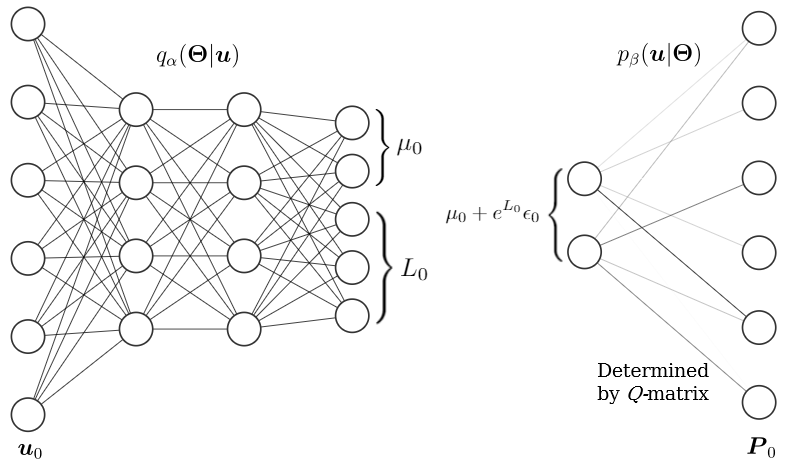
\includegraphics[width=.85\textwidth]{img/ml2pvae_visual.png}
  \caption{Visualization of the ML2P-VAE architecture for two correlated latent traits and six input items. Note that the trainable weights matrix in the decoder is not dense, but is determined by the given $Q$-matrix.}
  \label{fig:ml2pvae_visual}
\end{figure}

A visualization of the ML2P-VAE architecture for correlated latent traits is shown in Figure \ref{fig:ml2pvae_visual}. At test time, the estimate of the latent skills of a student with responses $\vect u_0$ is obtained via $\vect \Theta_0 = \vect \mu_0$. The output reconstruction $\vect P_0$ refers  to the reconstruction of the input $\vect u_0$, also interpreted as the probability of student $0$ answering each question correctly:
\[P_{i0} = P(u_{i0} = 1 | \vect \Theta_0; \vect a_i, b_i)\]



\subsection{Variants of ML2P-VAE}\label{sec:variants}

We consider three scenarios for using ML2P-VAE in practice: (a) the best case scenario where the covariance matrix between all latent traits is fully known, (b) the exact covariance matrix unknown, so it is estimated using other methods, and (c) we simply assume that all traits are independent. These three situations result in three variations of the ML2P-VAE method: ML2P-VAE$_{full}$, ML2P-VAE$_{est}$, and ML2P-VAE$_{ind}$, respectively. 

In order to estimate the correlations between latent traits for use of ML2P-VAE$_{est}$ in scenario (b), the student response matrix $U \in \R^{N\times n}$ is multiplied by the $Q$-matrix $Q \in \R^{n \times K}$. Denote $M = UQ \in \R^{N\times K}$. Then the Pearson correlation of the columns of $M$ produce an approximate correlation matrix $\hat \Sigma \in \R^{K \times K}$, where each entry $\hat \sigma_{kl}$ gives the approximate correlation between latent traits $k$ and $l$.
\begin{equation}
  \hat \sigma_{kl} = \frac{\sum_{i=1}^N (k_i - \bar k)(l_i - \bar l)}{\sqrt{\sum_{i=1}^N(k_i - \bar k)^2} \sqrt{\sum_{i=1}^N (l_i - \bar l)^2}}
  \label{eq:approx_cor_mat}
\end{equation}
where $\bar k$ and $\bar l$ are the mean values of the $k$-th and $l$-th columns of $M$, respectively.

A final variation of ML2P-VAE comes when the IRT model to be estimated is changed. If assuming that student responses are generated according to the Rasch model in Equation \ref{eq:rasch} rather than the ML2P model from Equation \ref{eq:ml2p}, then another variation of VAE parameter estimation methods can be considered. A more appropriate name for this alternative estimation method is Rasch-VAE.

Since there are no discrimination parameters in the Rasch model, only item difficulties and student abilities need to be estimated. To account for this, the weights in the VAE decoder are restricted to be \textit{equal} to the $Q$-matrix, i.e. $w_{ik} = q_{ik}$. This still allows for interpretation of the learned distribution of the VAE as estimates to student abilities $\vect \Theta$, while requiring ``discrimination parameters'' to be equal to either one or zero, fitting more closely to Equation \ref{eq:rasch}.

%
\section{\textbf{ML2Pvae} Software Package for R}
The ML2P-VAE method for parameter estimation has been compiled in an easy-to-use software package for R \cite{r_package}. This allows researchers who may not have experience with neural networks to implement ML2P-VAE methods on a data set of their choosing. The package \textbf{ML2Pvae} is available on the Comprehensive R Archive Network (CRAN) and can be easily installed using the R command:
\begin{lstlisting}[language=R, numbers=none]
install.packages('ML2Pvae')
\end{lstlisting}

\subsection{Package Functionality}
\textbf{ML2Pvae} uses Tensorflow and Keras to build and train neural networks, but no knowledge of these libraries are required in order to use \textbf{ML2Pvae}. The package exports five functions available to the user. Two of these are used to construct Keras models, with optional parameters specifying the architecture of the neural network. The only parameters which require input from the user are the number of items on the exam, the number of latent abilities that the exam assesses, and the $Q$-matrix relating items and abilities.

The optional inputs in the model construction include a covariance matrix for latent traits, allowing for correlated skills and the implementation described in Section \ref{sec:cov}. An important feature for model selection gives the choice of the number of item parameters to use in the logistic IRT model. Though the package is called \textbf{ML2Pvae} for the Multidimensional Logistic 2-Parameter model, the package allows for estimating parameters with the Rasch model, so that Rasch-VAE from Section \ref{sec:variants} can be implemented. In this case, there is only a difficulty parameter for each item; each  discrimination parameter is fixed to be equal to 1. Other options when building ML2P-VAE models specify the number, size and activation functions of the hidden layers in the encoder.

Using the Keras models returned by the construction functions, \textbf{ML2Pvae} provides a function that can be used to train the VAE on data. This function acts as a wrapper for the \verb!fit()! method in the Keras package. The final two methods obtain item parameter estimates and student ability parameter estimates. This is done by grabbing the correct weights/biases from the decoder and feeding student responses through the encoder, respectively. A more detailed description of the functionality of \textbf{ML2Pvae}, along with a code tutorial, is given in Appendix \ref{apdx:software}.

